\section{App implementation} \label{ch:app_implementation}

The prototype suffices as proof of concept.
However, the model lacks a suitable environment to be used.
The prototype applies the model and its implementation into each instance of \name{mec-2} and patches a canvas on top of the element to be able to draw.
This is not optimal, because this approach is neither flexible nor extensible.
So instead of using just the \name{mec2} HTML-element, a web application is built around it.
This web application may be used as a progressive web app to be accessed via a browser or even embedded into other third-party apps.

\subsection{Creation of a Progressive Web App}

The goal of the application is to provide a user interface where the user can work with \name{mec2} interactively, especially using hand-drawings.
This is achieved by using \name{mec2} as the base and creating an environment around this HTML-element.

Components used to create the user interface are mostly written using \name{React}. % TODO citation needed.
React is a JavaScript framework, which allows for the usage of single components, allowing standard HTML and JavaScript besides it.
This is a requirement the original \name{mec2} HTML-Component should be used without any modifications.

% TODO uncomment this. By using \name{materialUI} \cite{MaterialUI2020} a consistent and modern layout is created.

\subsection{Structure of the application}

\begin{figure}
    \centering
    \fbox{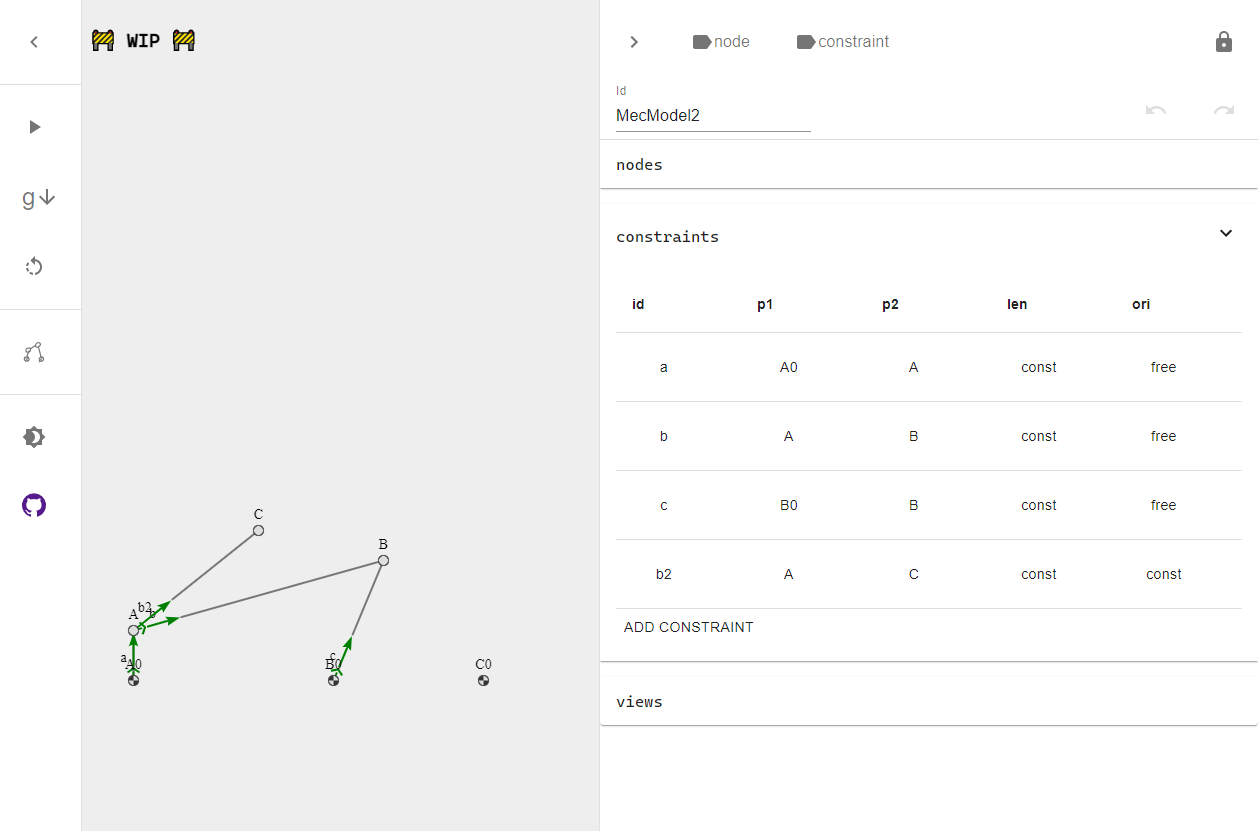
\includegraphics[width=0.8\textwidth]{images/deepmech_klawr_de.png}}
    \caption[Screenshot of the web application]{ Both drawers are expanded. On the left the \name{mec2} controls can be seen, on the right a summary of elements of the model are listed. The tab for \name{constraints} is expanded where some properties are shown }
    \label{fig:deepmech_klawr_de}
\end{figure}

\subsubsection{Left drawer}

The structure of the user interface aims to be simple and straight forward.
To define individual components \name{Reacts} \name{jsx} syntax is used.
\name{jsx} is a syntax very similar to \name{HTML} but with the ability to implement JavaScript into the elements\footnote{By using \name{jsx} it is now necessary to compile the project using \name{Babel.js}.}. % TODO citation neede

The left drawer contains \code{MecControl}, \code{DeepmechControl} and two other Buttons.
\code{MecControl} is a custom \name{React} component to replace the default \name{mec2} controls by using the designated API.

\begin{lstlisting}[label={lst:mec_control}, caption={Definition of the \name{MecControl component.}}]
export default function MecControl({ mecReset, className }) {
    const dispatch = useDispatch();
    const mec = useSelector(mecSelect);

    return <List className={className}>
        <ListButton onClick={() =>
            dispatch(mecAction.toggleRun())} tooltip="Run/Pause mechanism">
            {mec.pausing ? <PlayArrow /> : <Pause />}
        </ListButton>
        <ListButton onClick={() =>
            dispatch(mecAction.toggleGravity())} tooltip="Toggle gravity">
            g {mec.gravity ? <Clear /> : <ArrowDownward />}
        </ListButton>
        <ListButton onClick={mecReset} tooltip="Reset">
            <RotateLeft />
        </ListButton>
    </List>
}
\end{lstlisting}

Listing \ref{lst:mec_control} shows the function which returns the component replacing the default \name{mec2} controls.
It contains the definition of the variables \code{dispatch} and \code{mec}.
\code{Selector} and \code{useDispatch} are used for state management of the user interface and are examined in chapter \ref{ch:state_manipulation}.
The return value of a component is the contonent defined in \name{jsx} syntax.
\code{List} is a \name{Material-UI} component.
The list items inside the list are are implemented using \code{ListItems} containing a \code{Tooltip} and an \code{IconButton}.
To reuse \name{Material-UI} components multiple times without having to call them every time a custom \code{ListButton} component is used.
The code for \code{ListButton} can be reviewed at \aka{} % TODO include link here.

The left drawer also contains the \code{DeepmechControl}\footnote{\name{deepmech} is the current project name.}.
It is responsible for handling the draw mode.
It shows the activation button if the draw mode is disabled.
If the drawing mode is enabled the left drawer does not show the \code{MecControl} anymore.
Furthermore, the \code{DeepmechControl} shows four different modes interacting with the drawing canvas.
Drawing, dragging strokes, deleting strokes, and a camera mode.
Details to the different modes and how they are implemented is explained in chapter \ref{ch:state_manipulation}.

The two bottom-most buttons are responsible for toggling the dark mode\footnote{The app starts in dark mode if the browser is, and vice versa.} and to navigate to the project page: \url{https://github.com/klawr/deepmech}.

\subsubsection{Right drawer}

The right drawer is intended to show all information about the mechanism which is represented by \name{mec2}.
On the top, there are two buttons labeled \code{nodes} and \code{constraints} each with a \code{Label} icon.
Those are used to toggle the labels of \code{nodes} and \code{constraints} respectively.
The \code{Lock} Button is used to keep the drawer open when interacting with the model.
This is enabled by default if the side is wide enough; i.e. wider than 1200 pixels.

The model itself is contained within a \code{MecProperties} component.
The \code{MecProperties} component contains a collection of other custom components, individually created for the different properties of a \name{mec2} model.
The  first component is the \code{Id} component. It is showing the \code{id} property of the \name{mec2} model and updates it respectively on changes.

Currently three of the modules provided by \name{mec2} are implemented into the app.
\code{Nodes}, \code{Constraints} and \code{Views} show the associated properties.
They all follow a similar structure.


\subsubsection{The canvas}

\subsection{State manipulation} \label{ch:state_manipulation}

The state of the elements of the user interface is controlled by the 
